% This is samplepaper.tex, a sample chapter demonstrating the
% LLNCS macro package for Springer Computer Science proceedings;
% Version 2.20 of 2017/10/04
%
\documentclass[runningheads]{llncs}
%
\usepackage{graphicx}
% Used for displaying a sample figure. If possible, figure files should
% be included in EPS format.
%
% If you use the hyperref package, please uncomment the following line
% to display URLs in blue roman font according to Springer's eBook style:
% \renewcommand\UrlFont{\color{blue}\rmfamily}

\usepackage{cite}
\usepackage{amsmath,amssymb,amsfonts}
\usepackage{algorithmic}
\usepackage{graphicx}
\usepackage{textcomp}
\usepackage{xcolor}
\usepackage{float}
\usepackage{tikz}
\usetikzlibrary{shapes,arrows,decorations.pathmorphing,backgrounds,positioning,fit,petri,calc}
\usepackage[colorlinks,linkcolor=black,anchorcolor=black,citecolor=black, urlcolor=blue]{hyperref}
\usepackage{caption}
\usepackage{subcaption}
\usepackage{cleveref}
\captionsetup[table]{skip = 3pt}
\captionsetup[subfigure]{subrefformat=simple}
\usepackage{multirow}
\usepackage{booktabs}
\usepackage{etoolbox,siunitx}
\usepackage{array}
\newcolumntype{P}[1]{>{\centering\arraybackslash}p{#1}}

\tikzset{%
  every neuron/.style={
    circle,
    draw,
    minimum size=0.5cm
  },
  neuron missing/.style={
    draw=none, 
    scale=2,
    text height=0.333cm,
    execute at begin node=$\vdots$
  },
}

\begin{document}

%
% \title{Contribution Title\thanks{Supported by organization x.}}
\title{Article Template}
%
%\titlerunning{Abbreviated paper title}
% If the paper title is too long for the running head, you can set
% an abbreviated paper title here
%
\author{Hao Wen\inst{1,2}\orcidID{0000-0002-8856-0883}
% Wenjian Yu\inst{2} \and
% Yuanqing Wu\inst{1} \and
% % Lu Wang \inst{2} \and
% Jun Zhao \inst{2} \and
% Zhexiang Kuang \inst{2} \and
% Shuai Yang \inst{2}
% Xiaolong Liu \inst{2}
% Rong Fan \inst{2}
}
%
\authorrunning{H. Wen et al.}
% First names are abbreviated in the running head.
% If there are more than two authors, 'et al.' is used.
%
\institute{Tsinghua University, Beijing 100084, China \and
JingDong Health Inc., Beijing 101111, China
\email{\{wenh-06-10\}@tsinghua.edu.cn}\\
% \url{http://www.springer.com/gp/computer-science/lncs} \and
% ABC Institute, Rupert-Karls-University Heidelberg, Heidelberg, Germany\\
\email{\{wenhao71\}@jd.com}}


\maketitle


\setcounter{footnote}{0}

\begin{abstract}

\keywords{atrial fibrillation \and recurrent neural network \and convolutional neural network \and continuous monitoring.}

\end{abstract}

\section{Introduction}
\label{sec:intro}

\section{Related Work}
\label{sec:related_work}

\section{Method}
\label{sec:method}

\section{Experiments and Discussion}
\label{sec:experiments}

\section{Conclusions and Future Work}
\label{sec:conclusions_fw}


\section{Code availability}





\begin{figure}
\centering
\begin{subfigure}[b]{.4\textwidth}
\centering
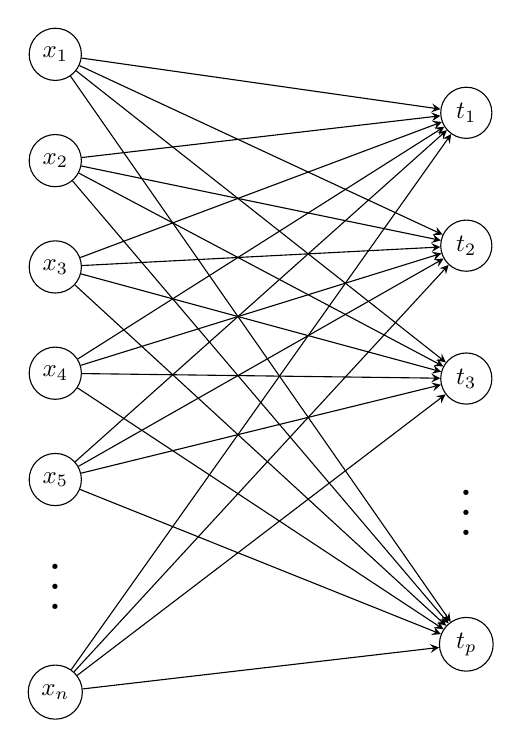
\begin{tikzpicture}[x=2.9cm, y=1.5cm, >=stealth, transform shape, scale=.9]

\foreach \m/\l [count=\y] in {1,...,5}
  \node [every neuron/.try, neuron \m/.try] (input-\m) at (0,3.5-\y) {$x_{\m}$};
  \node [neuron missing/.try] (input-missing) at (0,3.5-6) {};
  \node [every neuron/.try] (input-6) at (0,3.5-7) {$x_n$};

\foreach \h [count=\y] in {1,...,3}
  \node [every neuron/.try] (hidden-\h) at (2,3.2-\y*1.25) {$t_{\h}$};
  \node [neuron missing/.try] (hidden-missing) at (2,3.2-4*1.25) {};
  \node [every neuron/.try] (hidden-4) at (2,3.2-5*1.25) {$t_p$};

\foreach \i in {1,...,6}
  \foreach \j in {1,...,4}
    \draw [->] (input-\i) -- (hidden-\j);

\end{tikzpicture}
\caption{full connection}
\label{fig:full_con_nn}
\end{subfigure}\hfill
\begin{subfigure}[b]{.4\textwidth}
\centering
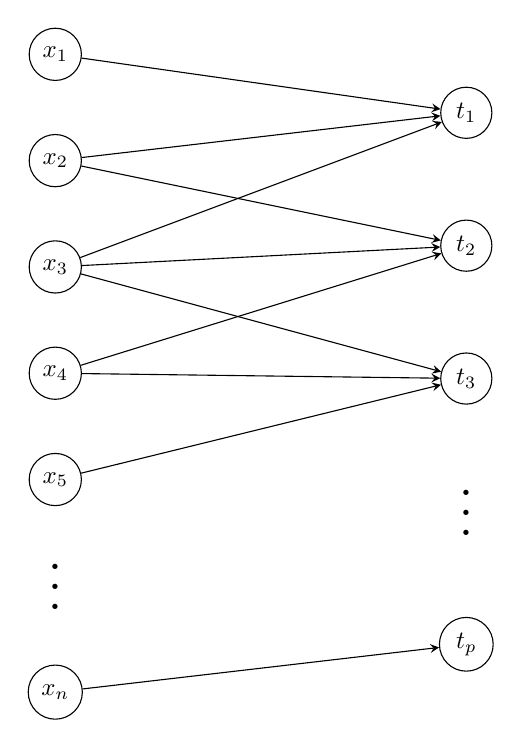
\begin{tikzpicture}[x=2.9cm, y=1.5cm, >=stealth, transform shape, scale=.9]

\foreach \m/\l [count=\y] in {1,...,5}
  \node [every neuron/.try, neuron \m/.try] (input-\m) at (0,3.5-\y) {$x_{\m}$};
  \node [neuron missing/.try] (input-missing) at (0,3.5-6) {};
  \node [every neuron/.try] (input-6) at (0,3.5-7) {$x_n$};

\foreach \h [count=\y] in {1,...,3}
  \node [every neuron/.try] (hidden-\h) at (2,3.2-\y*1.25) {$t_{\h}$};
  \node [neuron missing/.try] (hidden-missing) at (2,3.2-4*1.25) {};
  \node [every neuron/.try] (hidden-4) at (2,3.2-5*1.25) {$t_p$};

\foreach \i in {1,...,3}
    \draw [->] (input-\i) -- (hidden-1);
\foreach \i in {2,...,4}
    \draw [->] (input-\i) -- (hidden-2);
\foreach \i in {3,...,5}
    \draw [->] (input-\i) -- (hidden-3);
\draw [->] (input-6) -- (hidden-4);

\end{tikzpicture}
\caption{local connection}
\label{fig:local_con_nn}
\end{subfigure}
\caption{nn plot example}
\label{fig:nn}
\end{figure}



\bibliographystyle{splncs04}
\bibliography{references}
%
\end{document}
